\subsubsection{Example Based Super Resolution}
\noindent
Como puede observarse la interpolación soluciona parcialmente el problema de
\emph{Súper Resolución}, pero tiene como consecuencia los efectos mencionados. En
particular, el desenfoque resulta contraproducente al intentar mejorar los 
detalles de una imagen. Por lo mismo, en los algoritmos clásicos de \emph{Súper Resolución}
se utiliza la interpolación únicamente para aumentar la densidad de los pixeles
y aproximar la imagen de salida como una imagen más grande con un determinado 
factor de escalado, pero con los detalles de desenfoque que producen los 
algoritmos de interpolación no adaptativos. 

Para solucionarlo, algunos autores proponen realizar un postprocesado a la imagen 
interpolada para incluir los detalles faltantes y con ello mejorar visiblemente 
la calidad de los bordes de la imagen. 

En particular, \cite{freeman} propone un parchado de la imagen reescalada a partir
de un conjunto de entrenamiento o diccionario de parches en pares de alta
y baja resolución. Dichos parches permiten construir una imagen con frecuencias
altas que no están en la imagen de entrada con el objetivo de sumar la imagen
original interpolada con las frecuencias altas que buscan mejorar su resolución
al realzar sus detalles. En la Figura \ref{fig:fr_algoritmo} puede observarse de
manera específica el algoritmo propuesto basado en el parchado de la imagen de 
entrada mediante un algoritmo de predicción.

\begin{figure}[H]
    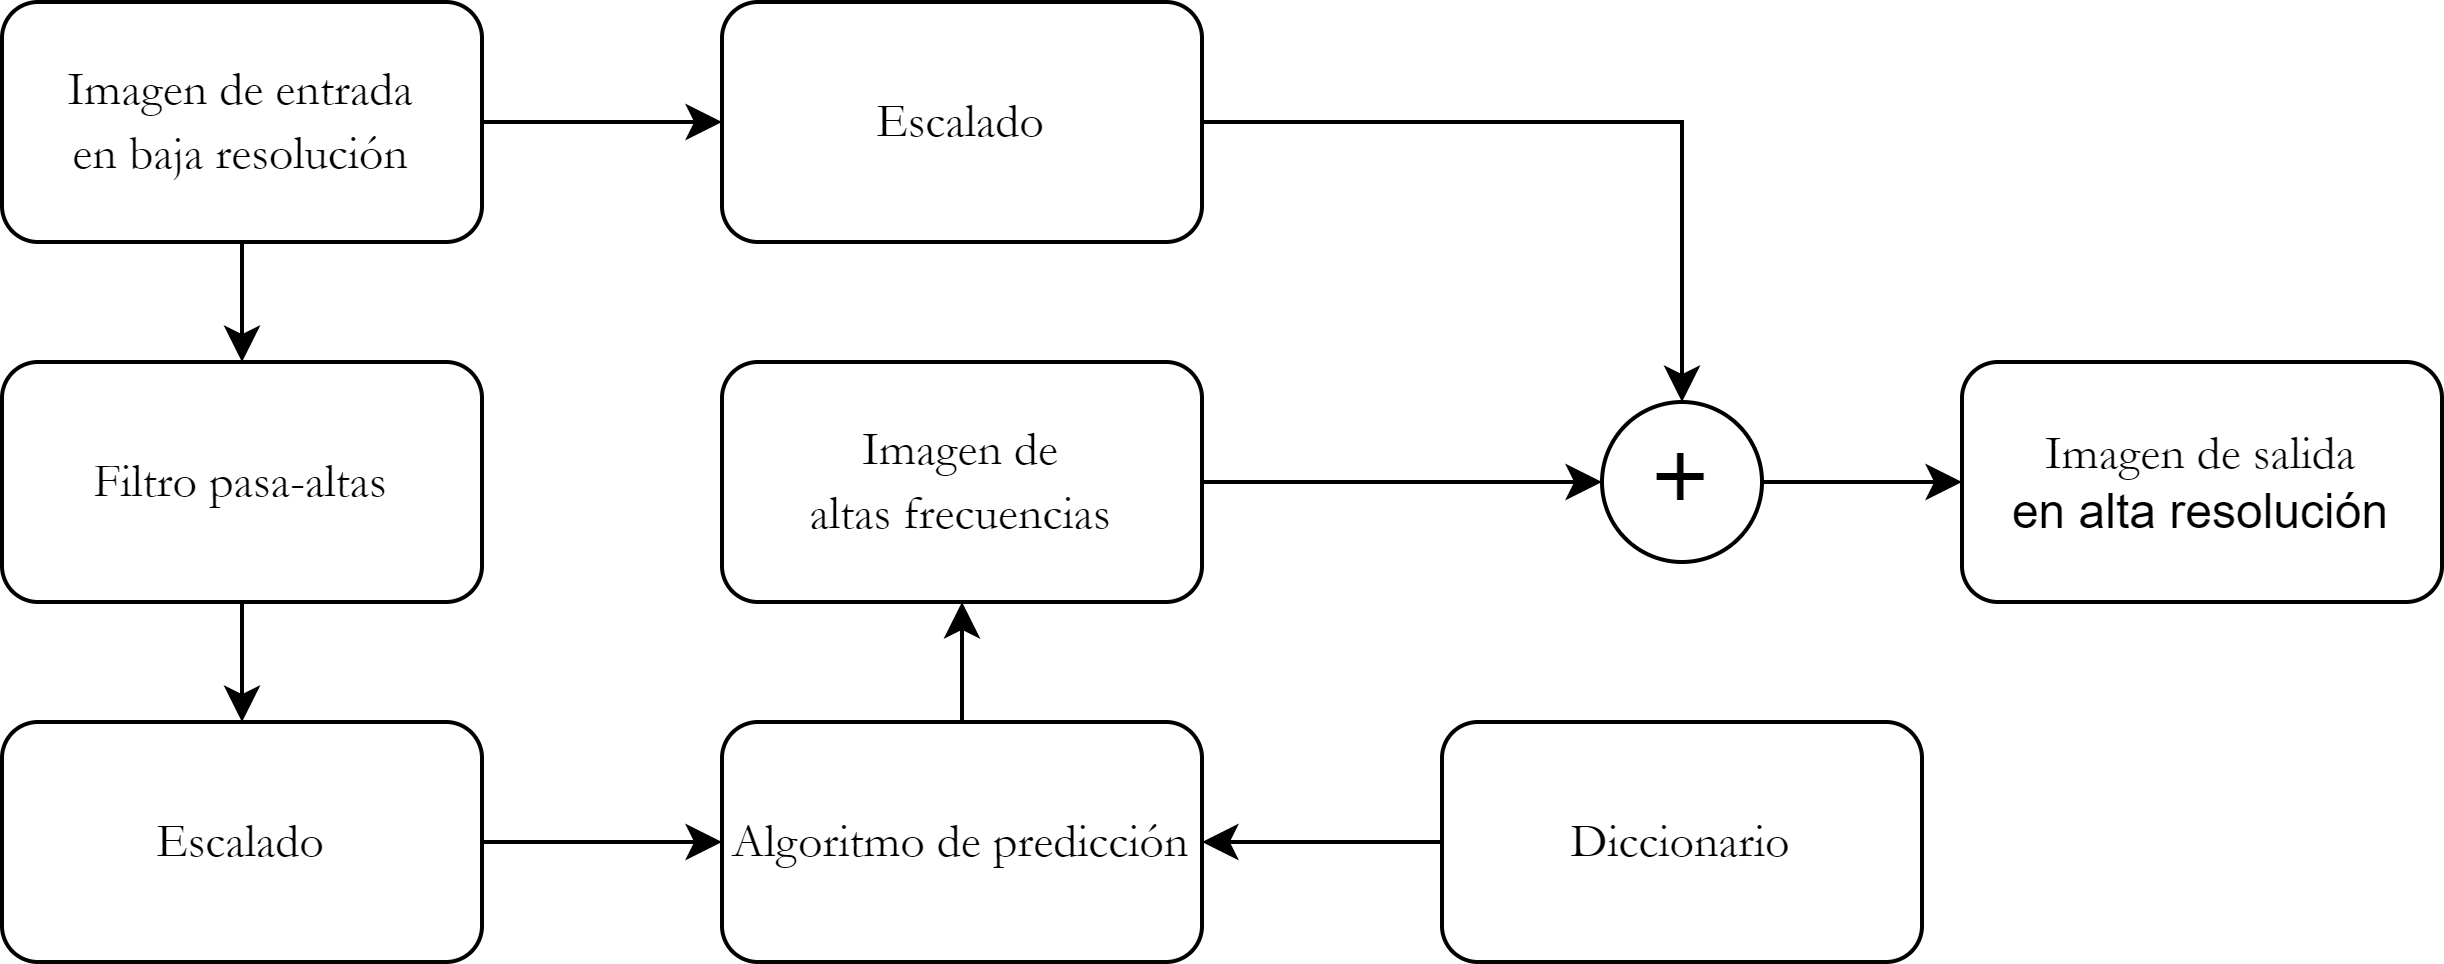
\includegraphics[scale = 0.8]{ fr_algoritmo.png }
    \centering
    \caption{ Algoritmo de súper resolución }
    \label{fig:fr_algoritmo}
\end{figure}

El algoritmo de \emph{Súper Resolución} propuesto por \cite{freeman}
opera bajo la premisa que la relación
de predicción entre los parches de alta y baja calidad es independiente del 
contraste de la imagen. Esto también resulta ventajoso, ya que el diccionario 
no necesita ser de imagenes similares a las que se van a reconstruir para 
mejorar la calidad de resolución similar a \cite{diccionario_shuji}.
Esto resulta en un algoritmo general aplicable a cualquier tipo de imagen. 

Para alcanzar esta generalidad es necesario normalizar los pares de los parches
mediante el promedio absoluto del parche de baja resolución correspondiente
a través de cada canal de color.